\documentclass[a4paper,11pt]{article}

\usepackage [utf8] {inputenc}
\usepackage [T1] {fontenc}
\usepackage [french b] {babel}

\usepackage{graphicx}

% package geometry pour la mise en page 
\usepackage{geometry} 
\geometry{scale=0.8, nohead} % definition des marges

\begin{document}

	\section{Introduction}
	
Dans le cadre de notre UV IA41 à l'UTBM, nous devions réaliser un projet de fin de semestre. Le choix du sujet s’est porté sur la création d'une intelligence artificielle pour un jeu vidéo. 
Dans le cas présent, il s’agit du jeu \texttt{Delirium 2}. Dans ce jeu, le joueur dirige un mineur se déplaçant dans des galeries souterraines à la recherche de diamants. Sur son parcours le mineur doit éviter un certain nombre de pièges, comme des monstres ou des rochers pouvant lui tomber sur la tête. Pour chaque souterrain, le joueur doit ramasser un certain nombre de diamant sur la carte pour ensuite se rendre à la sortie du niveau et passer au souterrain suivant.\\

Le but du projet est donc de rendre le mineur complètement autonome, ce dernier devant trouver seul son chemin pour récupérer les diamants, éviter les pièges et les ennemies qui l’entour puis rejoindre la sortie.\\

Ainsi, toutes les situations devront être étudiées pour que le mineur réponde intelligemment à celles-ci et fasse les choix les plus judicieux pour son évolution.\\

Nous allons vous présenter, à travers ce rapport, les différents problèmes que peut rencontrer le mineur et présenter les solutions que nous avons implémentées. Mais dans un premier temps, il est nécéssaire de constituer une spécification détaillée.
	
	\newpage
	\section{Spécifications}
	
La réalisation de la spécification s’est organisée par l’intermédiaire de réunions. Ces rencontres ont permis d'étudier les principes élémentaires requis pour une bonne évolution du mineur dans les souterrains. Ils nous on également permit de diviser notre travail en plusieurs partie. Chacune ayant pour rôle de répondre à un problème particulier.\\

Il est évident que pour réaliser ce projet il à fallu communiquer en dehors de ces séances. Un serveur de gestion de version à  été mis en place pour y déposé notre travail et une chaine de courriel à été utilisé pour la communication sur les différents états du projet.

Comme précisé en introduction, le jeu Délirium 2 met en situation un mineur devant évoluer dans des souterrains et répondant à certaines situations. Après analyse des différents niveaux déja implémentés dans le jeu de base, voici ce qui ressort de notre phase de spécifications :\\
		
		\begin{enumerate}
			\item Le mineur peut se déplacer dans 4 directions primaires (vers le haut, vers le bas, vers la droite, vers la gauche)
			\item Son déplacement d'une case A à une case B n'est possible que si la case B est de type "vide" ou "herbe"
			\item Son déplacement d'une case A à une case B est également possible si la case B est un rocher pouvant être déplacé.
			\item Une série de rochers (allant de 1 à N rochers) peut être déplacée si la case terminant la série de rocher et étant à l'opposée du mineur est de type "vide"
			\item Une série de rochers peut être déplacée vers la droite, vers la gauche ou vers le haut si elle répond aux points précédents.
			\item Son déplacement doit également prendre en compte des dangers pouvant provenir du haut.
			\item Un rocher peut tomber de sa position initiale si le mineur déplace une série de rochers inférieure, récupère un diamant ou creuse une case "herbe" qui soutenait le rocher.
			\item Le mineur peut récolter un diamant en position A, en arrivant des cases situées à gauche, à droite, en haut, ou en bas de la position du diamant.
			\item Cette règle peut être éronnée si le diamant est en cours de chute libre tout comme pourrait le faire un rocher (Cf : puce numéro 7). Dans cette situation le mineur ne peut pas récupérer le diamant par une case inférieure sinon il meurt.
			\item Le mineur peut rencontrer des ennemis le long de son parcours.
			\item Il y a 2 types d'ennemis que nous devons prendre en compte. Les monstres bleus et monstres rouges.
			\item Ces deux ennemis doivent être évités. C'est à dire que le mineur ne doit pas entrer dans un périmètre de deux cases autour du monstre.
			\item Un monstre ne peut se déplacer que d'une case "vide" à une case "vide".
			\item Certains monstre protègent des diamants. Le mineur doit dans certaines situations trouver une solution pour permettre de débloquer le diamant sans se faire attrapper par le monstre protégeant le diamant.
			\item Les monstres peuvent être tués si un rocher leur tombe sur la tête.
			\item Les souterrains peuvent contenir plusieurs types de "mur" infranchissable par les monstre et le mineur. Dans cet enssemble de mur existe des murs pouvant être détruits en faisant exploser un monstre à coté un certain nombre de fois (allant de 1 fois à 4 fois suivant le type de mur).
			\item Certaines situations contraignent le mineur à devoir provoquer la destruction d'un mur pour pouvoir débloquer un passage vers une autre partie du souterrain.
			\item Une carte de souterrain est définie par un fichier XML.
			\item Afin de terminer un niveau (ou souterrain), le mineur doit récolter un nombre de diamant minimum. Ce paramètre est définit dans le code XML de la carte.
			\item Le mineur est également contraint par un temps de jeu qu'il ne doit pas dépasser pour chaque niveau. Ce paramètre est également définit dans le code XML de la carte.
			\item Le mineur doit pouvoir trouver le diamant le plus proche dans son périmètre de vue.
			\item Le mineur doit pouvoir trouver le chemin le plus rapide d'un point A à un point B. En prenant en compte les élements cités précédement.
			\item Le mineur doit pouvoir abandonner un diamant qui ne sera jamais accessible. (Diamant entouré de mur par exemple.).
			\item Le mineur doit se concentrer sur la sortie dès que le nombre de diamants récoltés est égale au nombre de diamants nécéssaire pour terminer le niveau.
		\end{enumerate}
		
L'intelligence artificielle devra être développée grâce au langage Prolog. Il sera également préférable de séparer les différentes groupes de prédicats de même famille dans des modules prolog. Nous détaillons nos modules dans la partie réalisation de notre rapport.
	
	\newpage
	\section{Réalisation}
	
Différentes stratégies et algorithmes ont été développés pour répondre aux attentes de la phase de spécifications.  Qu’il s’agisse du déplacement, de la recherche d’un diamant, l’élimination d’un ennemi ou d'un passage rendu difficile par la chute de rocher ...\\

	\subsection{Recherche du plus court chemin : Algorithme A*}
	
Une solution avait été mise en place en début de projet, qui consistait à développer l'\texttt{Algorithme de Dijkstra}. Elle fut remplacée par une méthode plus adaptée à notre problème.
		
Cet algorithme reconnu de recherche de plus court chemin dans des graphes a été implémenté pour gérer les déplacements du mineur à partir d’un point de départ donné, d’un point d’arrivé et d’une liste représentant la carte du jeu. Il a été implémenté dans plusCourtChemin.pl. A partir de ces éléments l’algorithme étudie les directions possibles que peut prendre le mineur. Considérons la carte de jeu comme un tableau, chaque direction possible ajoute un lien entre la case où se trouve le mineur et celle où il peut aller, définissant ainsi un chemin possible. Tous les chemins possibles sont retenus dans une liste dite \textit{"ouverte"}, les chemins que le mineur ne peut pas prendre, comme par exemple un mur ou un rocher bloquant le passage, sont retenus dans une liste dite \textit{"fermée"}.  L’opération de recherche d’une direction possible est répétée à partir des chemins contenus dans la liste ouverte jusqu’à atteindre le point d’arrivée. Si un chemin s’avère être inefficace et n’abouti à rien, il sera à son tour inséré dans la liste fermée et retiré de la liste ouverte. Le chemin semblant être le plus court sera prioritaire et le mineur l’empruntera.

\begin{center}
\texttt{Complément d'informations à cette adresse : \\http:\/\/fr.wikipedia.org\/wiki\/Algorithme\_A*}
\end{center}

	\subsection{Stratégie de recherche du plus proche diamant}
	
		\subsubsection{Situation simple}
		
Dans le cas le plus simple, le mineur va chercher à aller au diamant le plus proche de lui. Par exemple sur la figure ci-dessous, le mineur va tracer son chemin vers le diamant numéro 1 puis se déplacer. Après ce déplacement il recherchera le dimant qui sera le plus proche de lui (à nouveau le 1) ; il se déplacera donc à nouveau dans la direction de ce diamant, et ainsi de suite…

		\begin{figure}[h]
			\center
			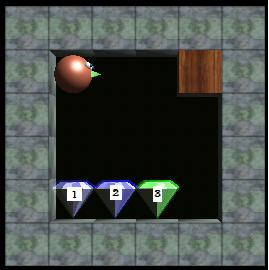
\includegraphics[width=5cm]{simple1}
			\caption{\label{simpleRechercheDiamant} Représentation d'une situation simple de recherche du plus proche diamant}
		\end{figure}
		
		\subsubsection{Situation plus complexe}
		
En réalité, il arrive très souvent que le diamant le plus proche du mineur soit inaccessible auquel cas on va préférer s’intéresser au diamant suivant. Par exemple sur la figure suivante, le diamant 1 est inaccessible, le mineur va alors rechercher au diamant numéro 2. Ce dernier étant également inaccessible, le mineur va alors se déplacer vers le diamant noté 3.
	
		\begin{figure}[h]
			\center
			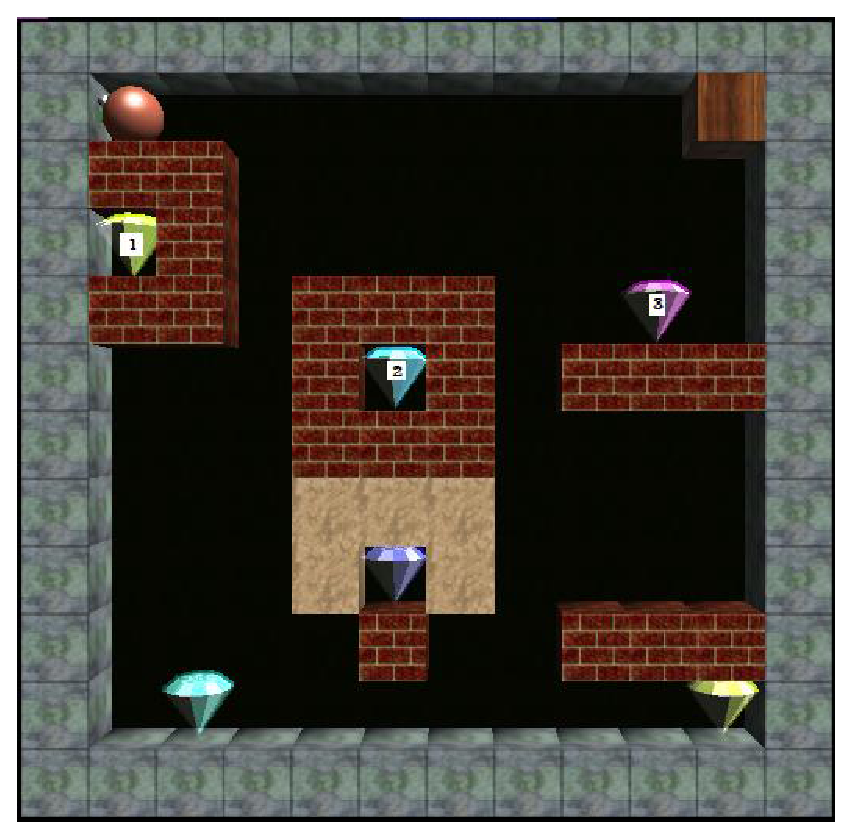
\includegraphics[width=9cm]{simple2}
			\caption{\label{complexeRechercheDiamant} Représentation d'une situation complexe de recherche du plus proche diamant}
		\end{figure}
		
	\newpage
	\subsection{Déplacement de rochers}
	
La stratégie de déplacement de rochers est très simple.\\
Tout d’abord il faut savoir que le mineur évite le plus possible de déplacer des rochers. S’il peut effectuer le déplacement sans déplacer de rochers, il le fera. Cette technique permet au mineur de ne pas bloquer stupidement ses objectifs. Par exemple sur la situation ci-dessous le mineur est tenté de partir sur la gauche à son premier déplacement auquel cas il bloquera la sortie. Grâce à l’utilisation du chemin sans déplacement de rochers, la sortie reste disponible.

		\begin{figure}[h]
			\center
			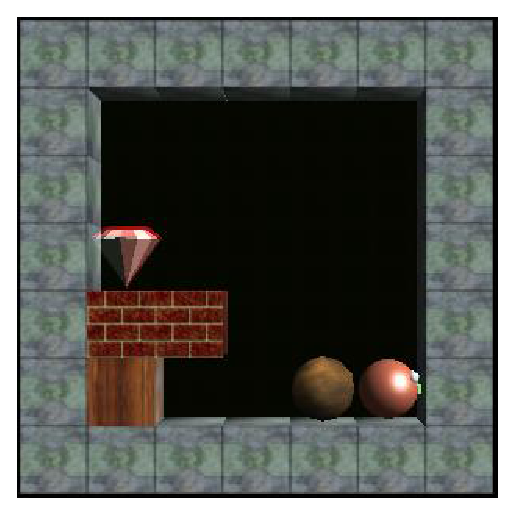
\includegraphics[width=5cm]{rochers1}
			\caption{\label{deplacementRocher1} Situation où le déplacement d'un rocher est possible mais pas nécéssaire}
		\end{figure}
		
Cependant le mineur est apte à déplacer les rochers ci cela devenait nécessaire, sur une profondeur choisit arbitrairement qui est de 5 rochers. Par exemple il peut pousser 5 rochers sur sa gauche si la situation s’y prête (pas d’obstacle derrière les rochers…). Par exemple dans la situation ci-dessous le mineur va bien évidemment déplacer les rochers pour se sortir de cette situation.

		\begin{figure}[h]
			\center
			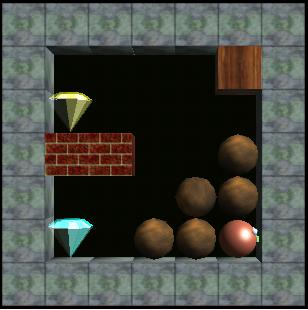
\includegraphics[width=5cm]{rochers2}
			\caption{\label{deplacementRocher2} Situation où le déplacement d'un rocher est obligatoire}
		\end{figure}
		
\newpage
Les rochers se déplacent parfois seuls, comme dans le cas d’une chute sur le mineur. Dans ce cas le mineur va alors détecter qu’il est menacé et il esquivera les rochers tombant en se décalant sur la gauche ou sur la droite selon les possibilités et l’objectif à atteindre.

		\begin{figure}[h]
			\center
			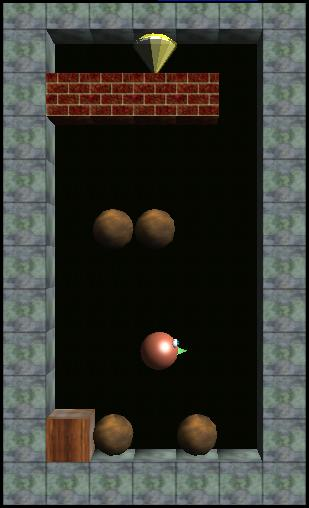
\includegraphics[width=5cm]{rochers3}
			\caption{\label{deplacementRocher3} Chute libre de plusieurs rochers sur le mineur}
		\end{figure}
		\clearpage
		
	\newpage
	\subsection{Stratégie mise en place pour éviter un monstre}
	
		\subsubsection{Cas général}
		
		Pour le cas général, dès que le mineur rencontre un monstre dans son champ de vision, la liste représentant le tableau de cases visibles par le mineur est modifiée avant de lui laisser chercher le plus court chemin vers le prochain diamant ou la sortie.\\
Chaque monstre présent dans le champ de vision du mineur est alors encerclé de murs à 2 cases aux alentours. L’algorithme A* recherchera donc un chemin lui permettant d’éviter le monstre. Bien entendu les murs ajoutés pour éviter le monstre ne sont pas visible pour le joueur.

		\begin{figure}[h]
			\center
			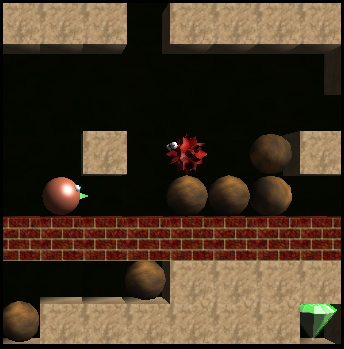
\includegraphics[width=5cm]{monstre1}
			\caption{\label{monstre1} Monstre mettant en danger le mineur : vision du joueur}
		\end{figure}
		
		\begin{figure}[h]
			\center
			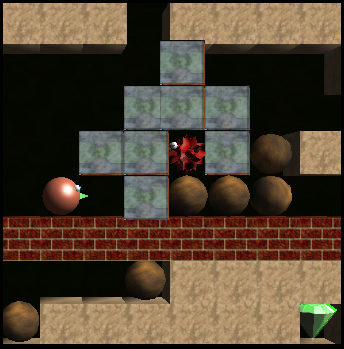
\includegraphics[width=5cm]{monstre2}
			\caption{\label{monstre2} Monstre mettant en danger le mineur : vision technique }
		\end{figure}
		
		\subsubsection{Cas plus complexe}
		
Afin de ne pas perturber l’environnement de la carte. Seules les cases accessibles par le mineur (case vide et case d’herbe) sont remplacées par des murs.
Mais nous aurions également pu avoir cette configuration :
	
		\begin{figure}[h]
			\center
			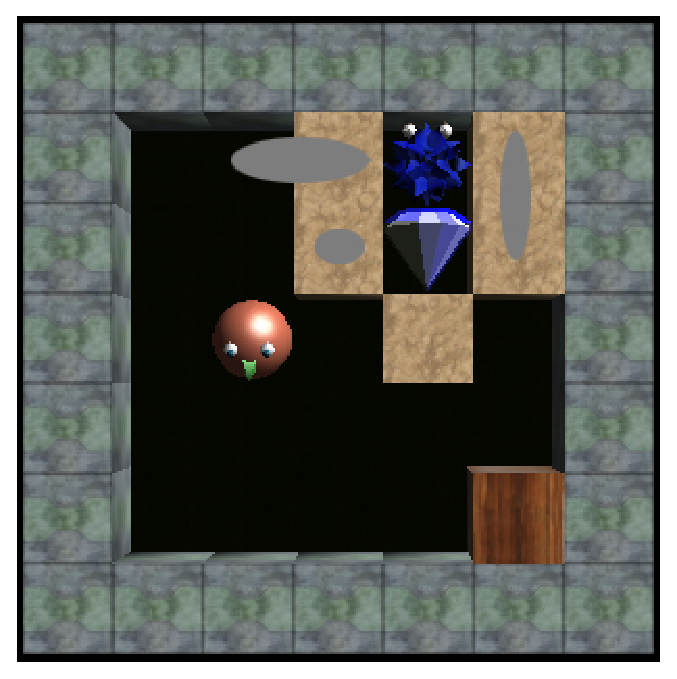
\includegraphics[width=5cm]{situation1}
			\caption{\label{monstre3} Limite de la construction de murs autour d'un monstre }
		\end{figure}
		
Sur cette représentation seules les cases marquées d’un marqueur gris seront remplacées par des murs. Le diamant n’est pas remplacé, ni la case herbe du dessous. Nous ne remplaçons donc pas la case de niveau supérieur à une case non remplacée. Ici la case herbe est au niveau 2 du champ de vision du monstre, le diamant au niveau 1 est bloquant pour la case herbe. La case herbe n’est donc pas remplacée.
Cette représentation nous permet de résoudre certaines situations.
	
	\newpage
	\subsection{Situation particulière 1 : Dimant piégé par un monstre}
	
		\subsubsection{Aperçu de la situation}
		
		Sur certaines cartes, un monstre peut bloquer l’accès au mineur à un diamant. Voici un aperçu de la situation :
		
		\begin{figure}[h]
			\center
			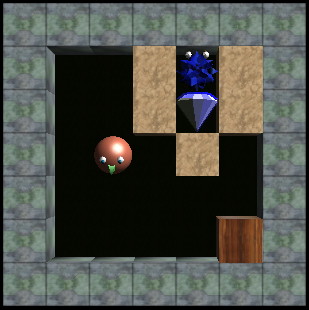
\includegraphics[width=5cm]{situation12}
			\caption{\label{situation1} Aperçu de la situation particulière 1 }
		\end{figure}
			
		\subsubsection{Résolution de la situation}
		
Afin de résoudre cette situation, le mineur devra creuser la case herbe située en dessous du diamant, puis s’écarter pour laisser tomber le diamant. L’algorithme standard de recherche du plus proche diamant et l’encerclement du monstre par des murs permettra ensuite au mineur de résoudre cette carte. Voici une image explicative de la solution :

		\begin{figure}[h]
			\center
			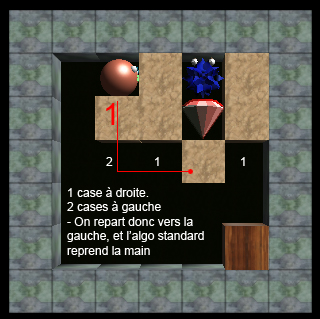
\includegraphics[width=5cm]{situation111}
			\caption{\label{situation1reso} Résolution de la situation particulière 1 }
		\end{figure}
	
	\newpage
	\subsection{Situation particulière 2 : Attaque des montres}
	
	Cette stratégie est implémentée dans situation2.pl. Elle consiste à neutraliser un ennemis dans une situation donnée que nous allons détailler par la suite. Elle se décompose en trois phases.

	\subsubsection{Phase 1 : repérer la situation}
	
La situation doit se présenter sous la forme suivante : un monstre se promène sur une ligne bloquée sur une courte distance. Au dessus de cette ligne se trouve une ligne d’herbe. Enfin, un rocher doit être présent au dessus de la ligne d’herbe en bout de course du monstre. La situation typique est résumée sur l’image ci-dessous.  
	
		\begin{figure}[h]
			\center
			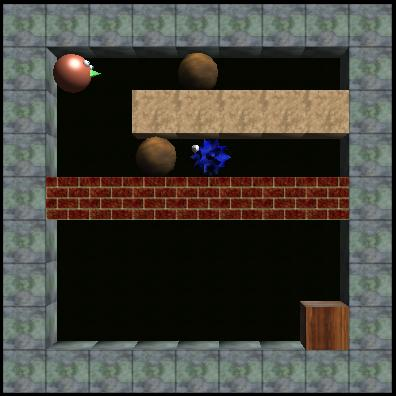
\includegraphics[width=5cm]{situation2-1}
			\caption{\label{situation21} Phase 1 de résolution de la situation 2 }
		\end{figure}
	
Cette situation étant repéré, le mineur va alors se mettre en position en sécurité comme sur l’image ci-dessous.
	 
		\begin{figure}[h]
			\center
			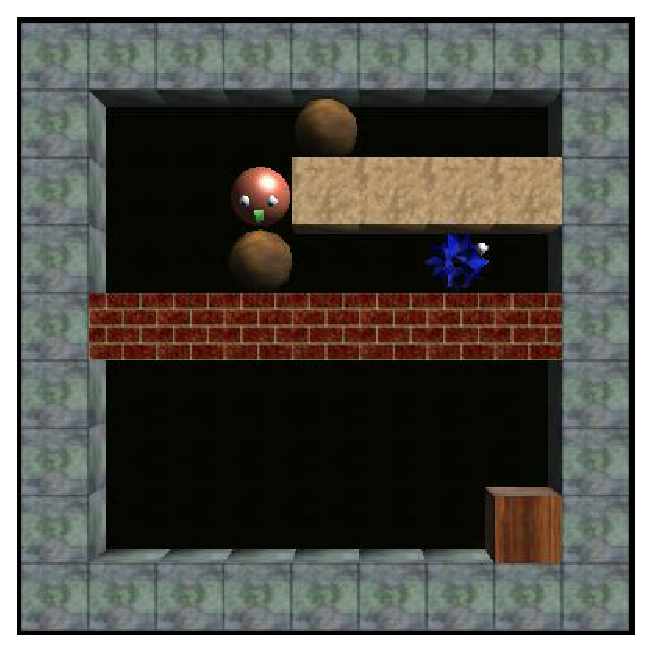
\includegraphics[width=5cm]{situation2-2}
			\caption{\label{situation22} Phase 1 de résolution de la situation 2 }
		\end{figure}
	 
	 \newpage
	\subsubsection{Phase 2 : placement sous le rocher}
	
Le mineur est à ce moment en position d’attente, il va alors attendre que le monstre se situe à quatre cases de distance à partir de sa butée à gauche pour se placer sous le rocher et se mettre en position d’attente, comme mis en image ci-dessous.

	\begin{figure}[h]
			\center
			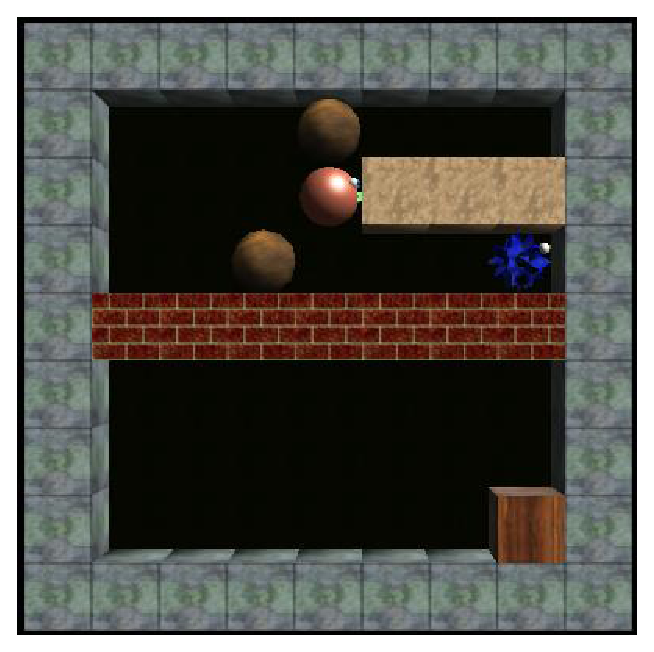
\includegraphics[width=5cm]{situation2-3}
			\caption{\label{situation22} Phase 2 de résolution de la situation 2 }
		\end{figure}
		
	\subsubsection{Phase 3 : Déclenchement du piège}
	
Enfin, lorsque le monstre s’approche, le mineur va s’écarter de sous le rocher de façon à ce que celui-ci tombe sur le monstre. Ainsi le monstre est neutralisé.

		\begin{figure}[h]
			\center
			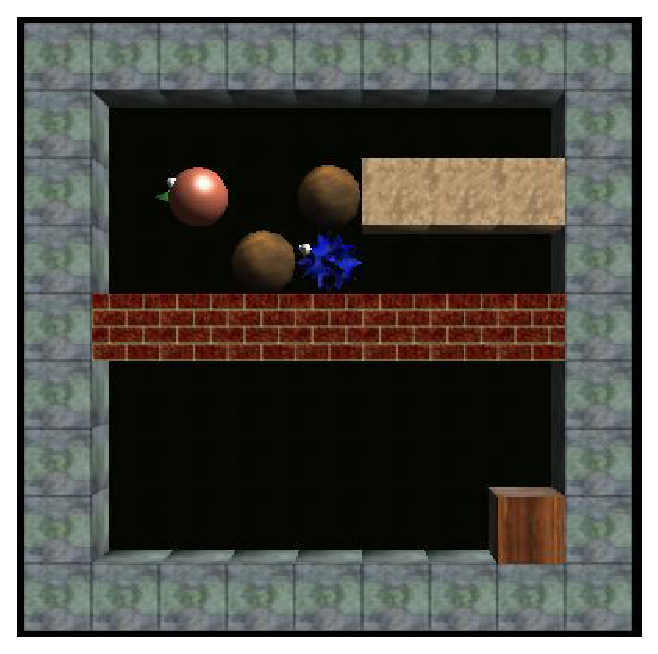
\includegraphics[width=5cm]{situation2-4}
			\caption{\label{situation22} Phase 3 de résolution de la situation 2 }
		\end{figure}
		
	\newpage
	\subsection{EXTRA : Editeur de carte Html/JavaScript}
	
Dès le début du projet, il nous était difficile de concevoir des cartes résumant une situation particulière. Nous n’arrivions pas à visualiser correctement ce que nous concevions comme carte dans le fichier XML. Nous avons donc pensé à concevoir un éditeur de carte Delirium 2.0 en HTML \/ JavaScript.

	\begin{figure}[h]
			\center
			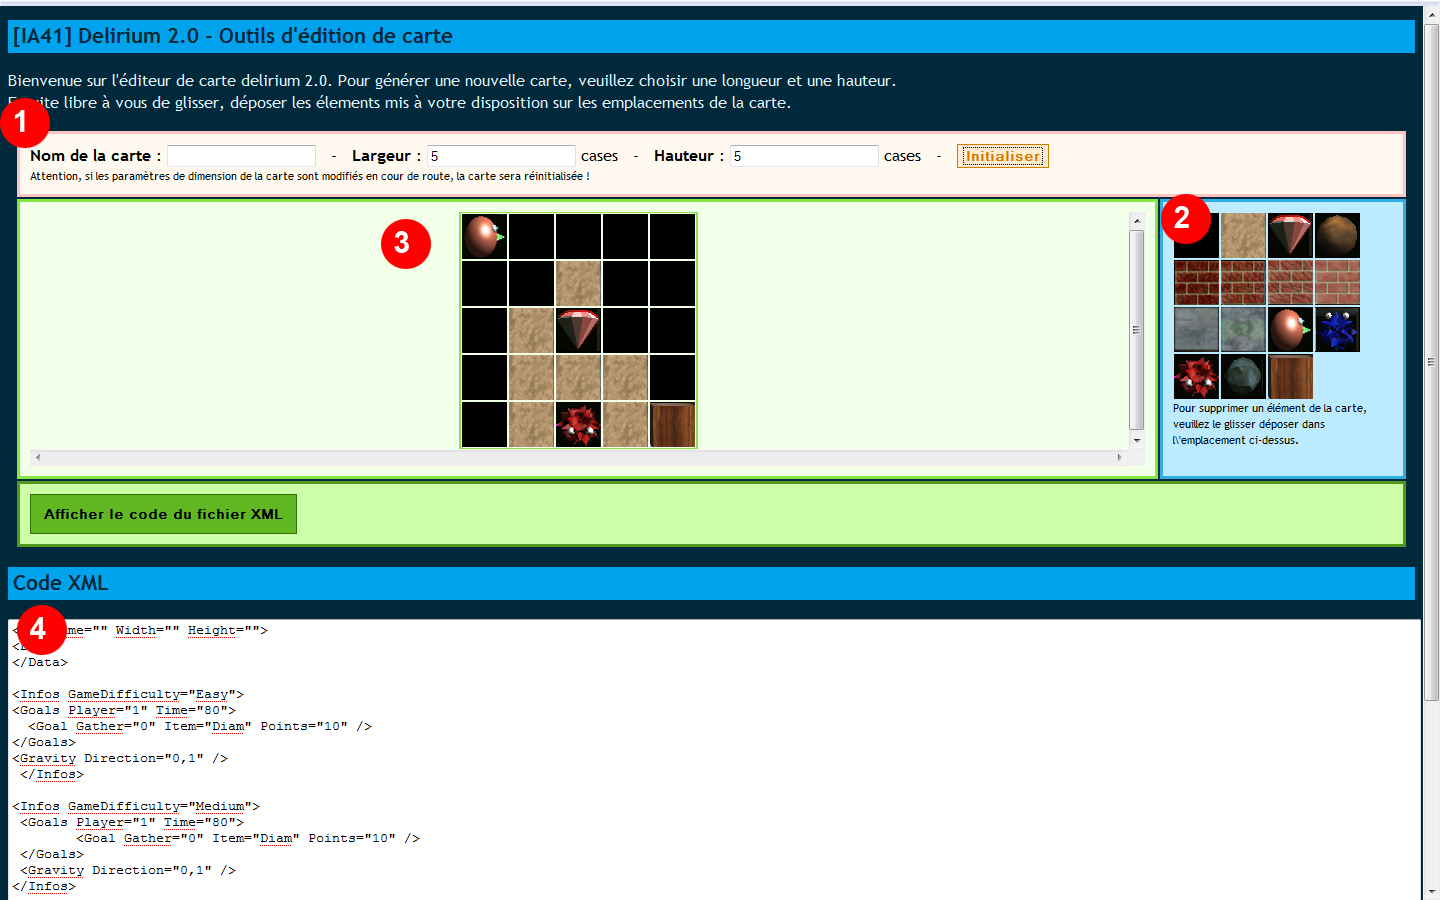
\includegraphics[width=12cm]{editeur}
			\caption{\label{situation22} Editeur de carte Delirium 2 }
		\end{figure}
		
	\begin{enumerate}
		\item Nous renseignons les informations de la carte
		\item Nous avons à disposition les éléments de la carte
		\item Nous pouvons glisser depuis le « 2 » les éléments de la carte sur la carte.
		\item Le code XML du fichier est généré automatiquement.
	\end{enumerate}
	
	\newpage
	\section{Conclusion}
	
Lors de ce projet de plusieurs mois, nous devions réalisation l’intelligence artificielle du héro d’un jeu vidéo, le permettant de se déplacer, de récupérer ses objectifs de mission, à savoir, des diamants, ainsi qu’éviter les ennemis qui le pourchassent et les pièges tendus par le décor et ses rochers. Aujourd’hui, notre héro est tout à fait capable de se débrouiller dans ce genre d’environnement, en prenant la direction des diamants et en évitant ou éliminant les ennemis, se servant même de l’environnement pour s’en sortir indemne. Les objectifs que nous nous étions posés ont donc été remplis.\\

De nombreuses difficultés ont été rencontrées, comme pour l’implémentation de l’algorithme A* qui est quelque peu délicat à programmer ou les situations d’esquive et d’élimination des ennemis. Travailler avec un langage récursif n’est pas non plus chose aisé au début.

Le travail que nous avons réalisé peut tout à faire être amélioré, notamment au niveau de la rapidité d’exécution qui est parfois assez lente, principalement lors de passages complexes ou de nombreux chemins sont possibles pour notre héro.  
	
	\newpage
	\tableofcontents

\end{document}